\begin{figure}[t]
\centering
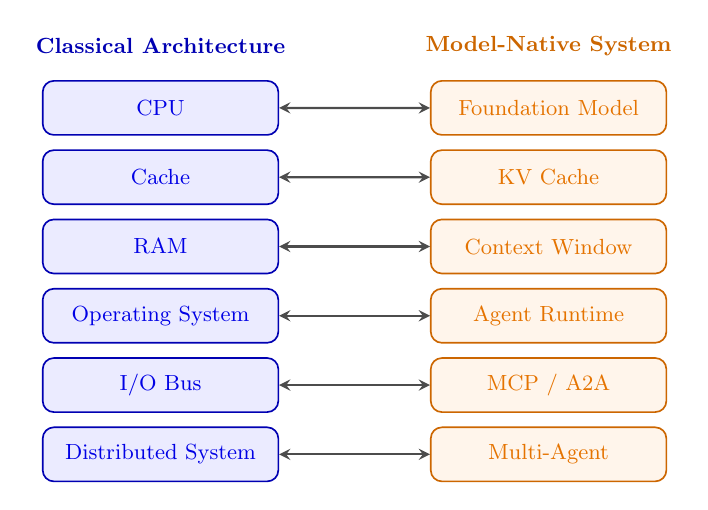
\begin{tikzpicture}[
    scale=0.88, every node/.style={transform shape},
    classicalbox/.style={
        draw=blue!70!black, fill=blue!8, rounded corners=4pt,
        minimum width=3.4cm, minimum height=0.78cm,
        font=\small, text=blue!90!black, align=center, line width=0.6pt
    },
    modelbox/.style={
        draw=orange!80!black, fill=orange!8, rounded corners=4pt,
        minimum width=3.4cm, minimum height=0.78cm,
        font=\small, text=orange!90!black, align=center, line width=0.6pt
    },
    coltitle/.style={
        font=\small\bfseries, align=center
    },
    arrowstyle/.style={
        <->, >=stealth, thick, gray!60!black
    }
]

% Column titles
\node[coltitle, text=blue!70!black] at (-2.8, 4.5) {Classical Architecture};
\node[coltitle, text=orange!80!black] at ( 2.8, 4.5) {Model-Native System};

% Classical column (left)
\node[classicalbox] (cpu)    at (-2.8, 3.6) {CPU};
\node[classicalbox] (cache)  at (-2.8, 2.6) {Cache};
\node[classicalbox] (ram)    at (-2.8, 1.6) {RAM};
\node[classicalbox] (os)     at (-2.8, 0.6) {Operating System};
\node[classicalbox] (bus)    at (-2.8,-0.4) {I/O Bus};
\node[classicalbox] (dist)   at (-2.8,-1.4) {Distributed System};

% Model-native column (right)
\node[modelbox] (fm)     at ( 2.8, 3.6) {Foundation Model};
\node[modelbox] (kv)     at ( 2.8, 2.6) {KV Cache};
\node[modelbox] (ctx)    at ( 2.8, 1.6) {Context Window};
\node[modelbox] (agent)  at ( 2.8, 0.6) {Agent Runtime};
\node[modelbox] (mcp)    at ( 2.8,-0.4) {MCP / A2A};
\node[modelbox] (multi)  at ( 2.8,-1.4) {Multi-Agent};

% Bidirectional arrows
\draw[arrowstyle] (cpu)   -- (fm);
\draw[arrowstyle] (cache) -- (kv);
\draw[arrowstyle] (ram)   -- (ctx);
\draw[arrowstyle] (os)    -- (agent);
\draw[arrowstyle] (bus)   -- (mcp);
\draw[arrowstyle] (dist)  -- (multi);

\end{tikzpicture}
\caption{Overview analogy mapping between computer architecture and model-native computing systems}
\label{fig_analogy_map}
\end{figure}
